% Copyright 2004 by Till Tantau <tantau@users.sourceforge.net>.
%
% In principle, this file can be redistributed and/or modified under
% the terms of the GNU Public License, version 2.
%
% However, this file is supposed to be a template to be modified
% for your own needs. For this reason, if you use this file as a
% template and not specifically distribute it as part of a another
% package/program, I grant the extra permission to freely copy and
% modify this file as you see fit and even to delete this copyright
% notice. 

\documentclass{beamer}

% There are many different themes available for Beamer. A comprehensive
% list with examples is given here:
% http://deic.uab.es/~iblanes/beamer_gallery/index_by_theme.html
% You can uncomment the themes below if you would like to use a different
% one:
%\usetheme{AnnArbor}
%\usetheme{Antibes}
%\usetheme{Bergen}
%\usetheme{Berkeley}
%\usetheme{Berlin}
%\usetheme{Boadilla}
%\usetheme{boxes}
%\usetheme{CambridgeUS}
%\usetheme{Copenhagen}
%\usetheme{Darmstadt}
%\usetheme{default}
%\usetheme{Frankfurt}
%\usetheme{Goettingen}
%\usetheme{Hannover}
%\usetheme{Ilmenau}
%\usetheme{JuanLesPins}
%\usetheme{Luebeck}
\usetheme{Madrid}
%\usetheme{Malmoe}
%\usetheme{Marburg}
%\usetheme{Montpellier}
%\usetheme{PaloAlto}
%\usetheme{Pittsburgh}
%\usetheme{Rochester}
%\usetheme{Singapore}
%\usetheme{Szeged}
%\usetheme{Warsaw}


% Customize Warsaw color 
\setbeamercolor*{palette primary}{use=structure,fg=white,bg=red!50!black}
\setbeamercolor*{palette secondary}{use=structure,fg=white,bg=red!60!black}
\setbeamercolor*{palette tertiary}{use=structure,fg=white,bg=red!70!black}

% Customize Warsaw block title and background colors
\setbeamercolor{block title}{bg=red!50!black,fg=white}


% List your packages here

\usepackage[colorinlistoftodos]{todonotes}


\title[Progress Update]{A Generalized Open Source Platform for Building Energy Management}

% % A subtitle is optional and this may be deleted
% \subtitle{Product Proposal}

\author[B.~Lauer]{Brian~Lauer\\\and
Advisor: Dr. Suruz Miah}
% - Give the names in the same order as the appear in the paper.
% - Use the \inst{?} command only if the authors have different
%   affiliation.

\institute[Bradley University] % (optional, but mostly needed)
{
  Department of Electrical and Computer Engineering\\
  Bradley University\\
  1501 W. Bradley Avenue\\
  Peoria, IL, 61625, USA
}
% - Use the \inst command only if there are several affiliations.
% - Keep it simple, no one is interested in your street address.

\date[September~3,~2020]{Thursday, September~3,~2020}
% - Either use conference name or its abbreviation.
% - Not really informative to the audience, more for people (including
%   yourself) who are reading the slides online

\logo{\hfill\href{http://www.bradley.edu}{
\includegraphics[width=0.75cm]{../figs/logoBU1-Print}}}  % place logo in every page 


\subject{Mobile Robot Localization}
% Section and subsections will appear in the presentation overview
% and table of contents.
\begin{document}
\begin{frame}
  \titlepage
\end{frame}

\begin{frame}{Outline}
  \tableofcontents
  % You might wish to add the option [pausesections]
\end{frame}
\section{Introduction}

\begin{frame}{Introduction}{}
  % applications of mobile robot navigation and problem description
  \begin{figure}
  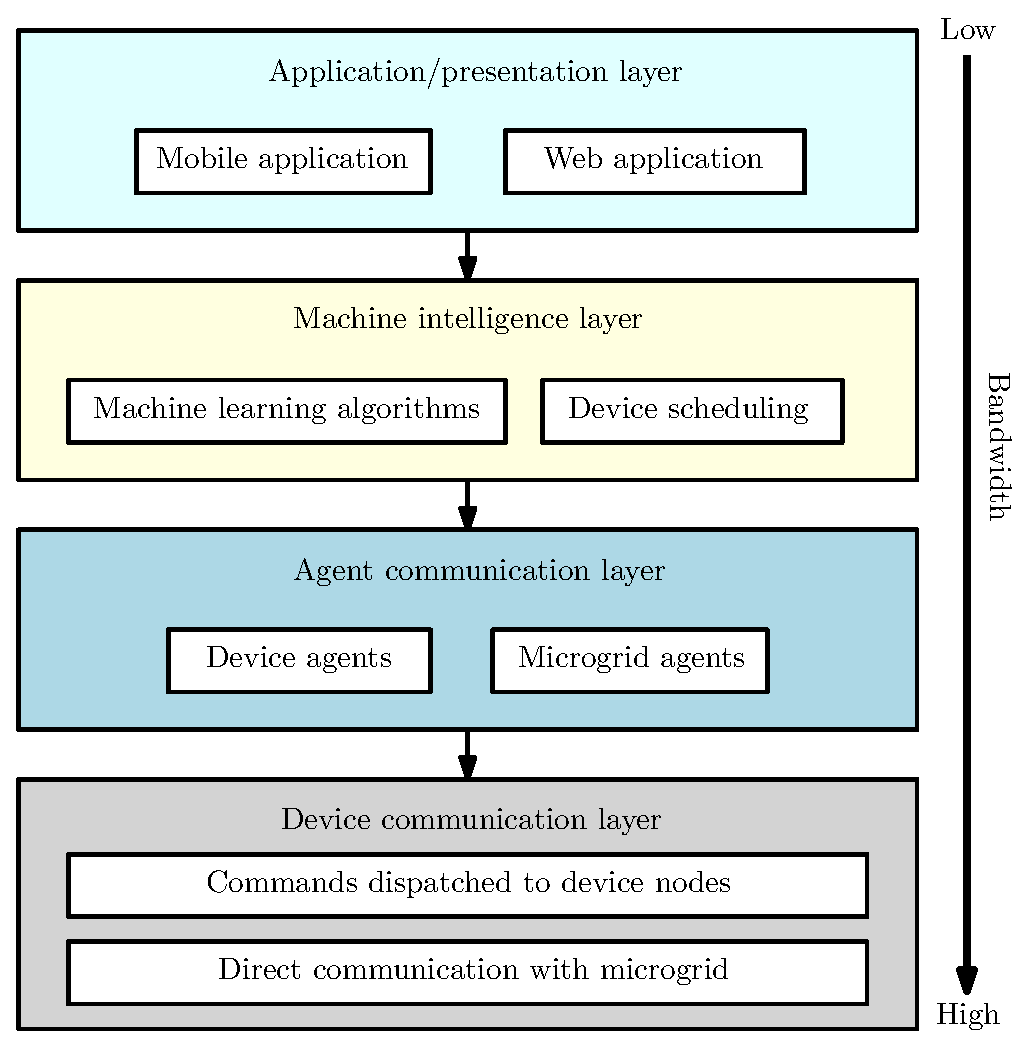
\includegraphics[scale=0.35]{../figs/ipe/BEMS-softwareArchitecture}
  \end{figure}
\end{frame}

\begin{frame}{Introduction}{}
  % applications of mobile robot navigation and problem description
  \begin{figure}
  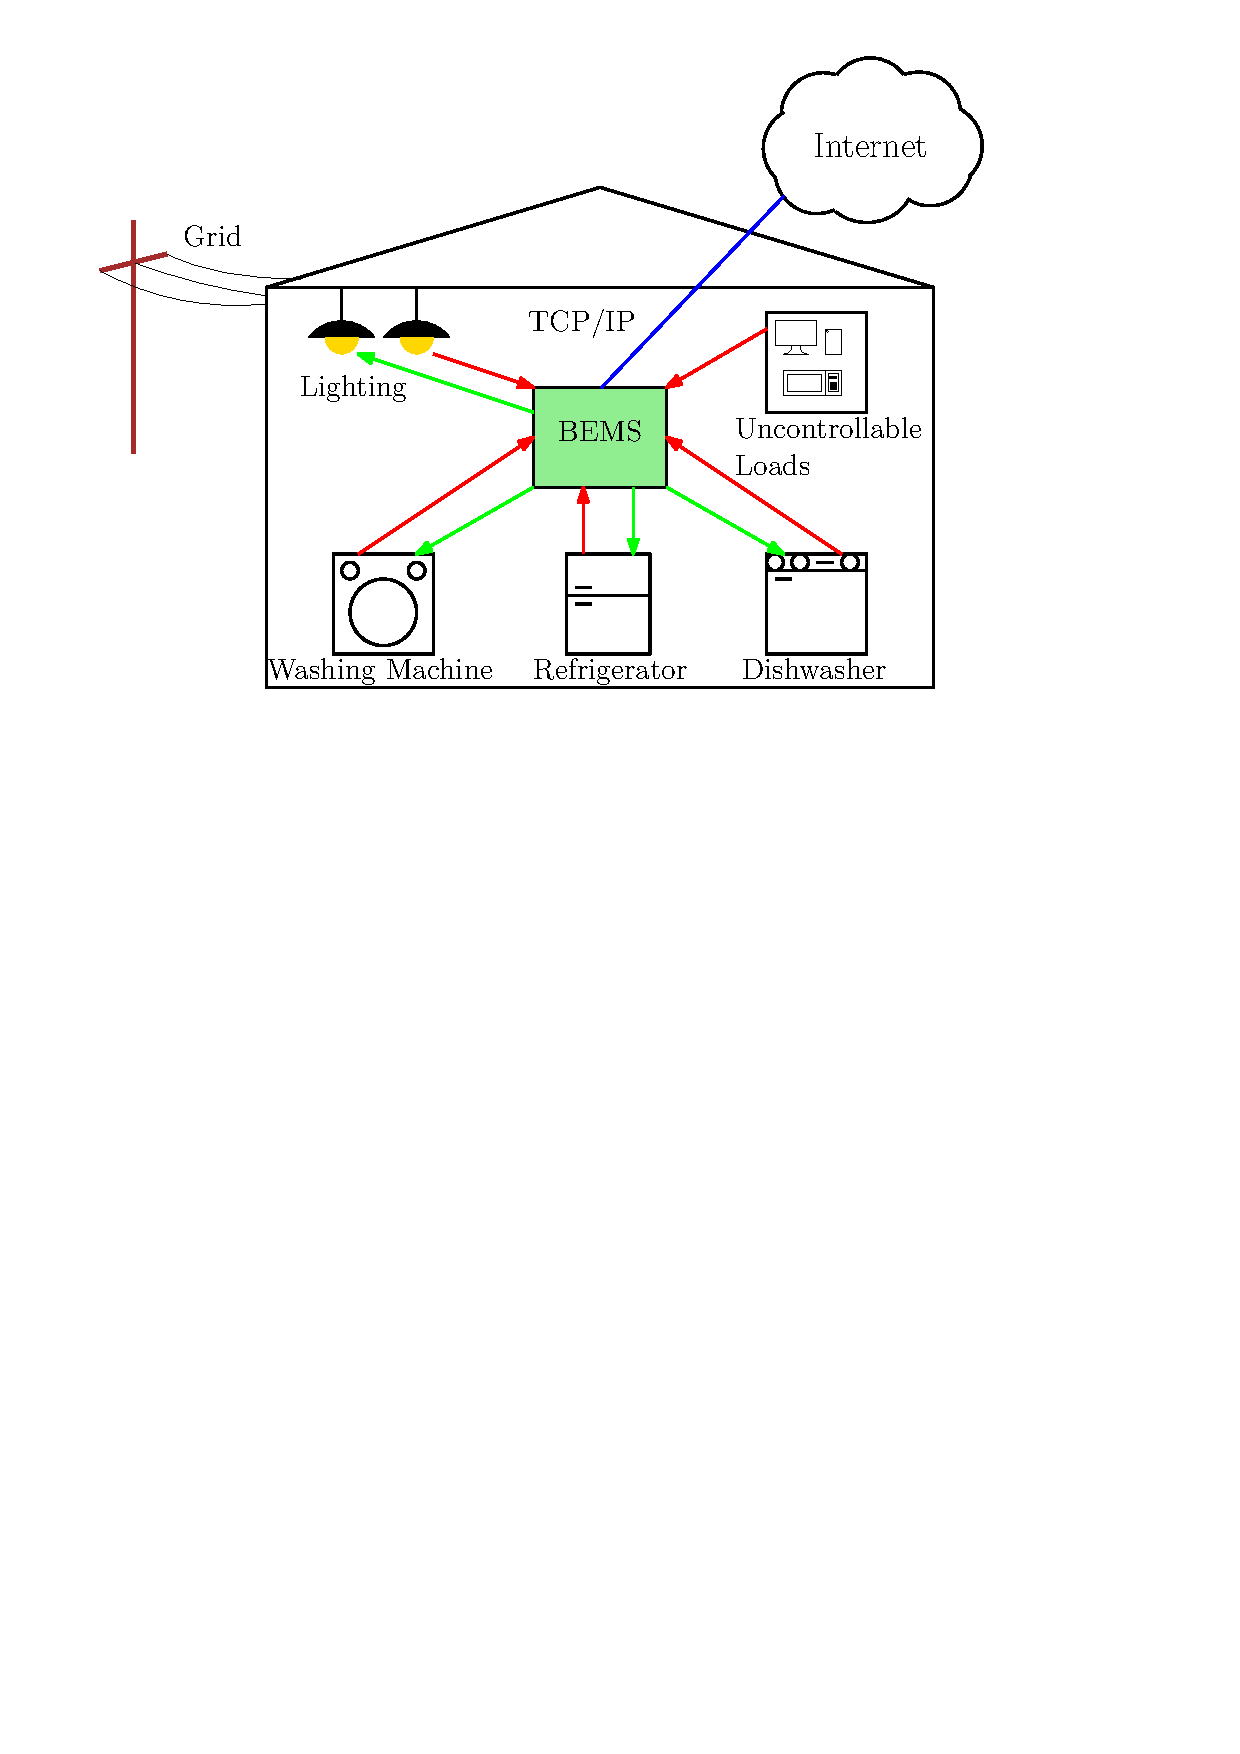
\includegraphics[scale=0.45]{../figs/ipe/bemsdiagram}
  \end{figure}
\end{frame}

\section{Progress}
\begin{frame}{Progress}{}
	\begin{itemize}
		\item Continued working on two functions added to \texttt{utils.py}, \texttt{insertIntoTSTable} and \texttt{createDeviceTSTable}
		\item For now, SQLite database will be used for storing time series database
	\end{itemize}
\end{frame}

\section{TS Table Creation}
\begin{frame}{TS Table Creation}{}
Steps followed in the algorithm: 
	\begin{enumerate}
		\item Select the contents of the \texttt{queryable} column in the \texttt{ActiveDevices} table corresponding to the device id passed as a parameter
		\item Split up the contents into individual strings, for example, 'power', and 'onOffStatus' for WeMoAPI
		\item Create a table titled \texttt{Device}[id number]\texttt{TSData} and add different columns corresponding to queryable values returned from \texttt{ActiveDevices} table, each column will be text data, the software should understand the names of these queryable values
	\end{enumerate}
	Note: deviceId is autoincremented when the devices is added to the \texttt{ActiveDevices} table
\end{frame}

\section{TS Table Insertion}
\begin{frame}{TS Table Insertion}{}
Steps followed in the algorithm
\begin{enumerate}
\item Retrieve the current time (month, day, year, hour, minute, second)
\item Create a time stamp string based on time data gathered from the above step
\item Check if a TS table for the device exists (for robustness and reliability purposes)
\item Check whether the last entry in the table was added greater than 40 minutes prior, if so remove the last entry in the table
\item Add the input data to the TS table (power, on/off data)
\end{enumerate}
\end{frame}

\section{Plans}
\begin{frame}{Plans}{}
\begin{itemize}
\item Finish working on working on the \texttt{insertIntoTSTable} function
\begin{itemize}
\item Determine how to check whether table exists in SQLite
\item Write parser for timestamp from previous entry
\item Find away to determine which table element was last added
\item Compare timestamps
\end{itemize}
\item Create an event loop in the \texttt{ControlAgent} to constantly poll data from the device
\item Add UI element for displaying power consumption and on/off status
\end{itemize}
\end{frame}


\begin{frame}
\Huge
\center
Any Questions?
\end{frame}
\end{document}


%%% Local Variables:
%%% mode: latex
%%% TeX-master: "../progressPresMain"
%%% End:
